\documentclass{article}
\makeatletter
\renewcommand{\fnum@figure}{Εικόνα \thefigure}
\makeatother
\usepackage[greek, english]{babel}
\usepackage{alphabeta}
\usepackage{atbegshi, picture}
\usepackage[letterpaper,top=2cm,bottom=2cm,left=3cm,right=3cm,marginparwidth=1.75cm]{geometry}
\usepackage{amsmath}
\usepackage{graphicx}
\usepackage[colorlinks=true, allcolors=blue]{hyperref}
\usepackage[utf8]{inputenc}
\usepackage{indentfirst}
\usepackage[table]{xcolor}

\addto\captionsenglish{
  \renewcommand{\contentsname}
    {Περιεχόμενα}
}

\newcommand\T{\rule{0pt}{2.6ex}}       % Top strut
\newcommand\B{\rule[-1.2ex]{0pt}{0pt}} 

\begin{document}



\begin{titlepage}
   \begin{center}
       \vspace*{1cm}

       \textbf{\huge Domain Model v0.2}

       \vspace{0.5cm}
        Τεχνολογία Λογισμικού
            
       \vspace{1cm}

       \textbf{Βεργίνης Δημήτριος\\Βλαχογιάννης Δημήτριος}
       
       \begin{figure}[!htb]
        \centering
        
\includegraphics[width=0.5\textwidth]{logo.jpg}
        \end{figure}
        
        \vspace{0.5cm}
        
        \begin{figure}[!htb]
        \centering
        
\includegraphics[width=0.5\textwidth]{ceid.png}
        \end{figure}


       \vfill
            
       Τεχνικό Κείμενο για την Τεχνολογία Λογισμικού\\
            
       \vspace{0.5cm}
            
       CEID, ECE\\
       University of Patras\\
            
   \end{center}
\end{titlepage}

\noindent Η ομάδα μας

\begin{enumerate}
  \item Βεργίνης Δημήτριος, ΑΜ: 10166634 , ECE
  \item Βλαχογιάννης Δημήτριος, ΑΜ: 1067371, CEID
  \item Κούρου Αγγελική, ΑΜ: 1067499 , CEID
  \item Μητροπούλου Αικατερίνα - Quality Manager, ΑΜ: 1067409, CEID
  \item Στεφανίδης Μάριος - Project Manager, ΑΜ:1067458, CEID
\end{enumerate}
{
  \hypersetup{linkcolor=black}
  \tableofcontents
}

\section{Περιγραφή}
Στο παρακάτω κείμενο θα γίνει μια αρχική παρουσίαση των κλάσεων που θα απαρτίζουν τον σχεδιασμό του \textbf{Medic World}. Για περαιτέρω βοήθεια στην κατανόηση πρέπει να γίνουν οι εξής διευκρινίσεις:
\begin{itemize}
    \item Με απλή γραμμή συμβολίζουμε την απλή συσχέτιση μεταξύ των κλάσεων.
    \item Με το τρίγωνο παρουσιάζουμε τις σχέσεις κληρονομικότητας.
    \item Η γραμμή με τον άδειο ρόμβο αναπαριστά την σχέση συνάθροισης.
    \item Ο μαύρος ρόμβος συμβολίζει σχέσεις σύνθεσης.
\end{itemize}

\begin{figure}[!htb]
        \centering
        \includegraphics[width=0.5\textwidth]{arrows.png}
\end{figure}
\newpage
\section{Domain Diagram}
Παρακάτω φαίνεται το αρχικό σχήμα του domain model.


\begin{figure}[!htb]
        \centering
        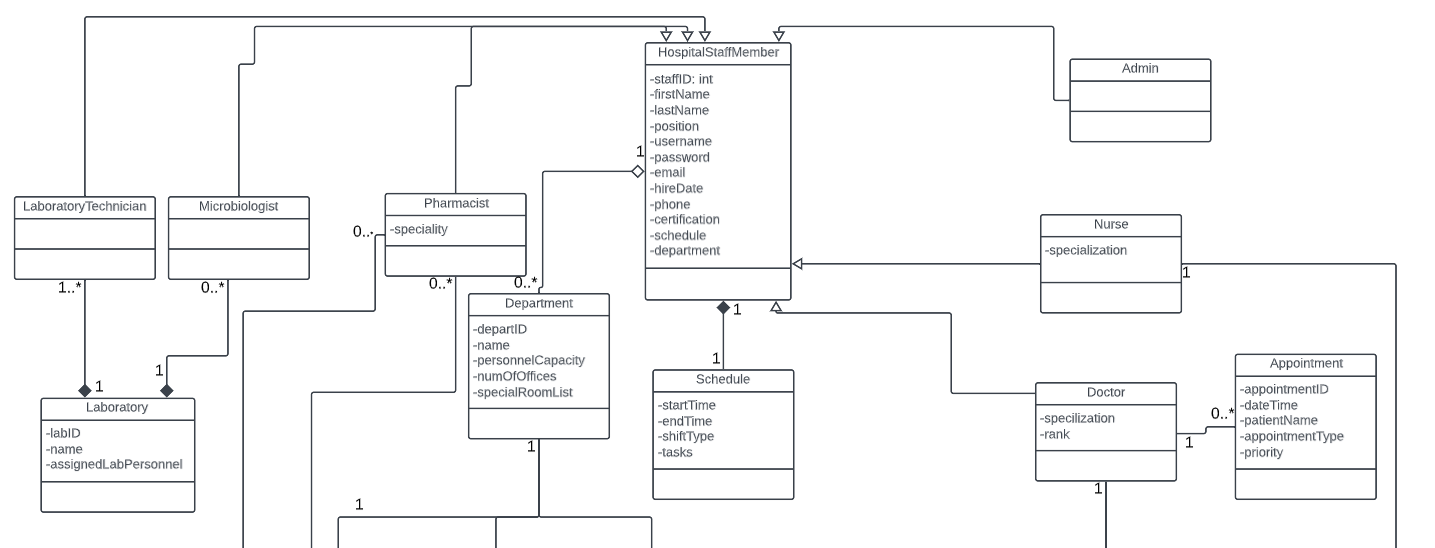
\includegraphics[width=1\textwidth]{domain1.png}
\end{figure}
        
\begin{figure}[!htb]
        \centering
        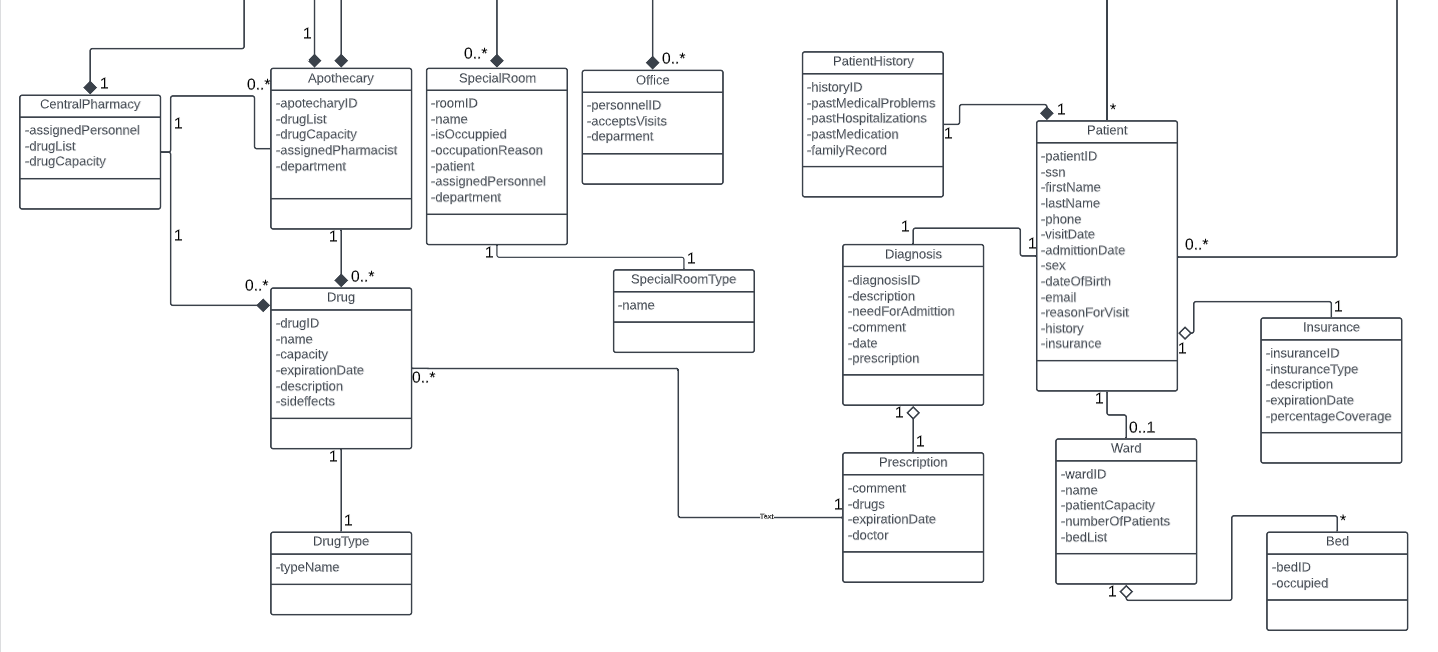
\includegraphics[width=1\textwidth]{domain2.png}
\end{figure}
        


\section{Ανάλυση κλάσεων}

\begin{itemize}
    \item \textbf{HospitalStaffMemeber}: Είναι η βασική οντότητα που περιέχει όλο το προσωπικό του νοσοκομείου, περιλαμβάνει ιδιότητες μοναδικές για κάθε άτομο (π.χ. ονοματεπώνυμο, αφμ, μισθός κ.α.).
    \item \textbf{LaboratoryTechnician}: Ειδίκευση της οντότητας του προσωπικού. Υπεύθυνος για τη λειτουργία του Laboratory (εργαστηρίου).
    \item \textbf{Microbiologist}: Ειδίκευση της οντότητας του προσωπικού. Υπεύθυνος για τις μικροβιολογικές εξετάσεις.
    \item \textbf{Pharmacist}: Ειδίκευση της οντότητας του προσωπικού. Υπεύθυνος διαχείρισής της οντότητας Apothecary (φαρμακείου).
    \item \textbf{CentralPharmacy}: Κεντρικό φαρμακείο του νοσοκομείου από το οποίο προμηθεύονται όλα τα Apothecary.
    \item \textbf{Department}: Οντότητα που αναπαριστά τα διάφορα τμήματα του νοσοκομείου (π.χ. Ενδοκρινολογικό, Ακτινολογικό).
    \item \textbf{Laboratory}: Τμήμα του νοσοκομείου οπού αναλύονται τα δείγματα του κάθε ασθενή και προκύπτουν τα μικροβιολογικά αποτελέσματα. 
    \item \textbf{Apothecary}: Συστατικό μέρος του τμήματος, περιλαμβάνει όλα τα απαραίτητα για την εύρυθμη λειτουργία της υπηρεσίας, φάρμακα.
    \item \textbf{Drug}: Οντότητα που περιέχει τις γενικές πληροφορίες για το κάθε φάρμακο (ημ.παραλαβής, απόθεμα) καθώς και σε ποιον ασθενή έχει συνταγογραφηθεί.
    \item \textbf{DrugCategory}: Κλάση που περιέχει το είδος του κάθε φαρμάκου και τη χρήση που αυτό θα έχει (αντιφλεγμονώδες, αντιπυρετικό κ.α).
    \item \textbf{OperatingRoom}: Αποτελεί το χειρουργείο μέσα στο νοσοκομείο και δηλώνει αν αυτό είναι διαθέσιμο για χρήση.
    \item \textbf{Office}: Οντότητα που αναπαριστά το γραφείου του προσωπικού.
    \item \textbf{Schedule}: Αποκλειστικό πρόγραμμα για κάθε ένα από τους υπαλλήλους, το οποίο δεν είναι σταθερό.
    \item \textbf{Doctor}: Ειδίκευση της οντότητας του προσωπικού, συσχετίζεται με τους ασθενείς.
    \item \textbf{Patient}: Κλάση που περιέχει όλες τις βασικές πληροφορίες για τον ασθενή.
    \item \textbf{PatientHistory}: Ειδική οντότητα που περιλαμβάνει το ιστορικό του ασθενή (παλαιότερες επισκέψεις, ασθένειες, κληρονομικότητα).
    \item \textbf{Diagnosis}: Η διάγνωση του ασθενή που προκύπτει από την εκάστοτε επίσκεψη του ασθενούς στο νοσοκομείο και την εξέταση από το γιατρό.
    \item \textbf{Prescription}: Η συνταγογράφησή του γιατρού προς τον ασθενή εφόσον αυτή κριθεί απαραίτητη από την εξέταση.
    \item \textbf{Ward}: Οντότητα που αναπαριστά την πτέρυγα του νοσοκομείου στην οποία βρίσκεται ο ασθενής εφόσον έχει εισαχθεί.
    \item \textbf{Room}: To δωμάτιο στο οποίο βρίσκονται οι ασθενείς.
    \item \textbf{Nurse}: Ειδίκευση της οντότητας του προσωπικού, μια νοσοκόμα μπορεί να είναι υπεύθυνη για παραπάνω από έναν ασθενή.
    \item\textbf{Admin}: Ο διαχειριστής του νοσοκομειακού συστήματος υπεύθυνος για την τεχνική συντήρηση της εφαρμογής. Έχει πρωτεύοντα ρόλο στην εφαρμογή παρά την παρανοσοκομειακή φύση της εργασίας του.
    \item\textbf{Message}: Κλάση που αποθηκεύει τις πληροφορίες για το εκάστοτε μήνυμα μεταξύ των μελών του νοσοκομείου.
    \item\textbf{Event}: Κλάση που αναπαριστά την εκδήλωση που μπορεί να φτιάξει κάποιος χρήστης της εφαρμογής.
    \item\textbf{Post}: Οντότητα που να περιλαμβάνει τις πληροφορίες για μια ανάρτηση ενός μέλους του προσωπικού στην πλατφόρμα της εφαρμογής.
    \item\textbf{Examination}: Οι εξετάσεις που ο γιατρός συνταγογραφεί σε έναν ασθενή.
    \item\textbf{CarePlan}: Αποτελεί όλο το πλάνο θεραπείας του ασθενούς καθ' όλη την διάρκεια της διαμονής του στο νοσοκομείο.
    \item\textbf{Procedure}: Επεμβάσεις στις οποίες μπορεί να υποβληθεί ο ασθενής.
    \item\textbf{Disease}: Οι διάφορες ασθένειες με τις οποίες μπορεί να διαγνωσθεί ο ασθενής.
\end{itemize}



\end{document}
